% 26.04.2024
\section{$\frac{3}{5}$ spanners}

\begin{df}[Multiplication Spanner] \label{df:mul_spanner}
  $H$ is a $k$-spanner of $G$ if $H \subseteq G$($H$ is a subgraph defined by set of edges) and

  \begin{align*}
  \forall u, v \in V(G) \implies d_H(u, v) \leq k \cdot d_G(u, v)
  \end{align*}

  , here $d(u, v)$ is a distance between $u$ and $v$.
\end{df}

\begin{remrk}[Hitting sets] \label{df:hitting_sets}
	Suppose $t$ sets $S_1, S_2, \ldots, S_t \subseteq \mathcal U$, where $\forall i \in [t]$ we have $|S_i| \geq q$ and $|\mathcal U| = n$.

	Let $T$ be a random subset of $\mathcal U$(universe) of size $k$, such that

	\begin{align} \label{eq:hitting_k}
		\Pr[\forall i \in [t] \; S_i \cap T \neq \varnothing] =  1 - \Pr[\exists i \colon S_i \cap T = \varnothing] \approx 1 - t \cdot \left(1 - \frac q n\right)^{k}
	\end{align}, for small $k$.

	In Eq. \eqref{eq:hitting_k} if $k \approx \frac{\alpha \cdot n \cdot \ln (t n) + 1}{ q }$ for some constant $\alpha \in > 1$, then 

	\begin{align*}
		1 - t \cdot \left(1 - \frac q n\right)^k \leq 1 - t e^{- \frac{k q}{n}} = 1 - t e^{-\alpha \ln(t \cdot n) + 1} \leq 1 - e n^{-\alpha}
	\end{align*}

\end{remrk}

\begin{lm}[folklore]
Let $H$ be subgraph of $G$ and $\forall (u, v) \in E(G) \implies d_H(u, v) \leq k$, then $H$ is a $k$-spanner of $G$.
\end{lm}

\begin{proof}
  Each path in $G$ is a set of edges, so if statement satisfies for every edge, then it satisfies for any path.
\end{proof}



\begin{thm}
	We are given a graph $G$(current graph) and have some updates(add / delete an edge).

	We can construct $3$-spanning tree $H$ of size $O\left(n^{\frac{3}{2}}\sqrt{\log n}\right)$ in time TODO.
\end{thm}

\begin{remrk} (Idea)
We would randomly construct an oriented version of $\vec G$, simply putting random orientation on every edge.

After that we would keep two graphs $A \subseteq G \setminus \tilde B$ and $B \subseteq \vec G$.
And our invariant is $H = A \cup \tilde B$, where $\tilde B$ is a graph where each orientation is deleted(in some words, $A$ would keep vertices of large degree and $B$ vertices of small degree).
And $H$ would be $3$-span of $G$ on first $4 n^3$ updates. And $H$ has small amount of edges.
\end{remrk}

\begin{proof}
	\begin{lm}[Alg1] \label{lm:spanning_alg_1}
	  There exists and algorithm for constructing 3-spanning TODO
	\end{lm}
	\begin{proof}
	  
  Let $S_1, \ldots, S_k \in V$. Initially we take them at random.
  It would be a centers of our clusters. Initially we put vertex to cluster if cluster center is it's neighbour(so some vertices is out of clusters) and put it's edge to cluster to $A$.
  We call $C_i$ cluster with center $S_i$.

  If a vertex of graph $G$ has some edge to another cluster, we would save in $A$ an edge from that vertex to center of another cluster.

  And also we put an edge $(u, v)$ in $A$, if $(u, v) \in \vec G \setminus B$ and $u \in C_i$ such that $u$ is minimum(lexicographically) and $v$ can be anywhere.  See Fig. \eqref{fig:proof_spanning_u_v}.

  \begin{figure}[H]
  	\centering
  	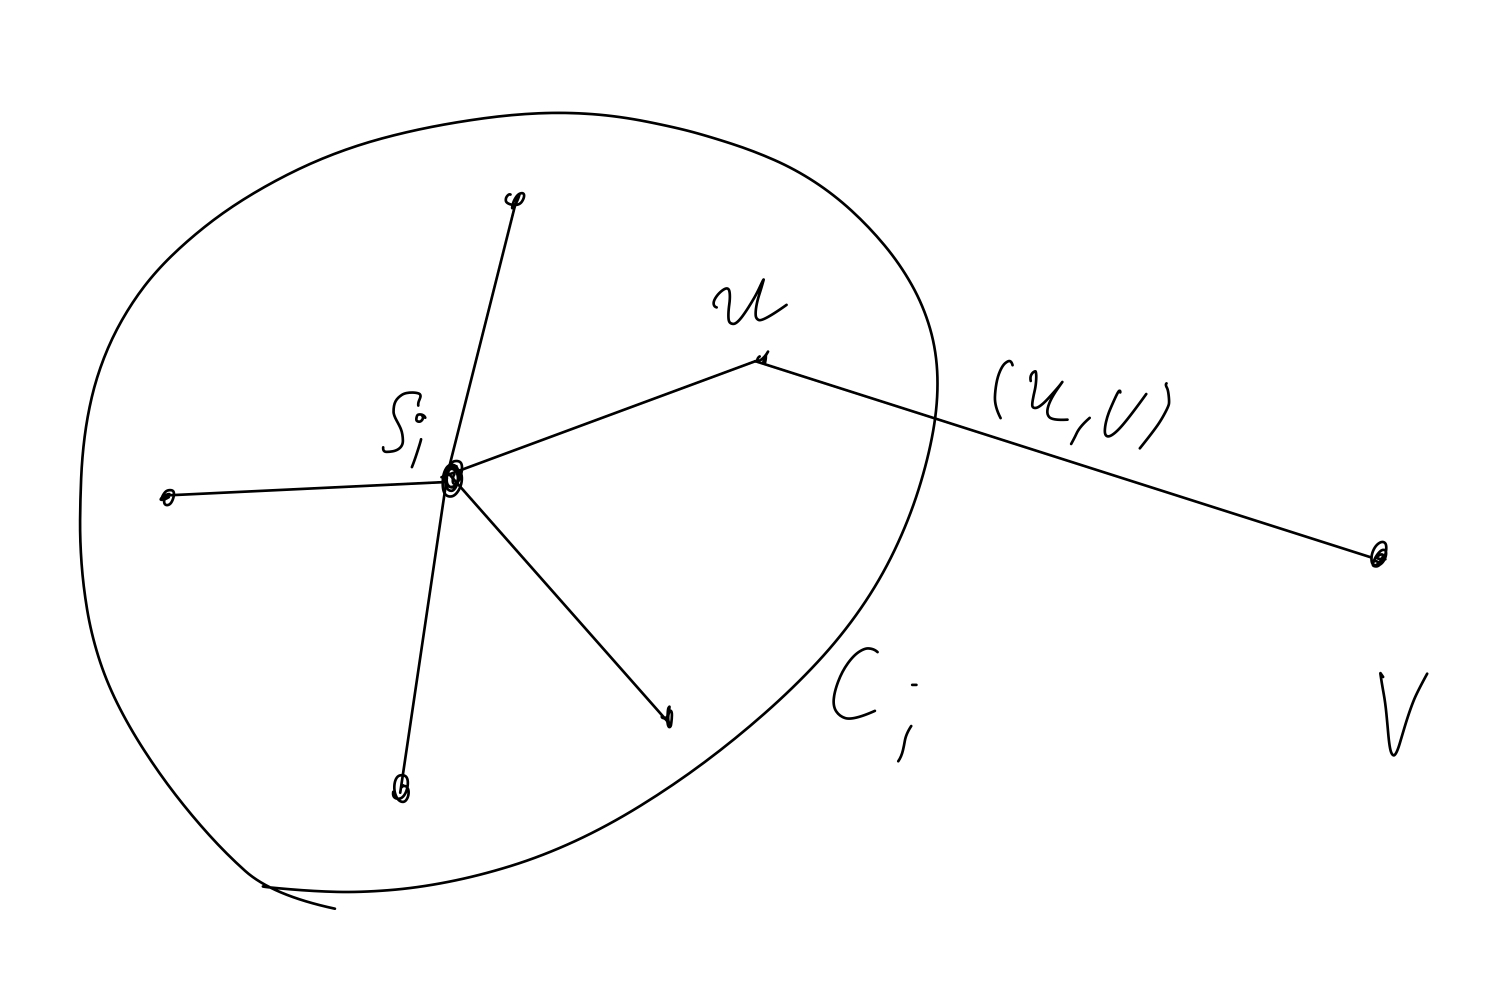
\includegraphics[width=0.5\linewidth]{figures/proof_spanning_u_v.jpeg}
  	\caption{Cluster.}
  	\label{fig:proof_spanning_u_v}
  \end{figure}

  Now, if $(u, v) \in E(G \setminus \tilde B)$ and let $v \in C_i$ and $\deg^{out}_{\vec G \setminus B}(v) > q$.
  Then, if there is an edge $(v, u) \in E(\vec G \setminus B)$, then there is exists and yellow edges.
  See Fig. \ref{proof_spanning_oriented_cluster_yellow}.

  \begin{figure}[H]
  	\centering
  	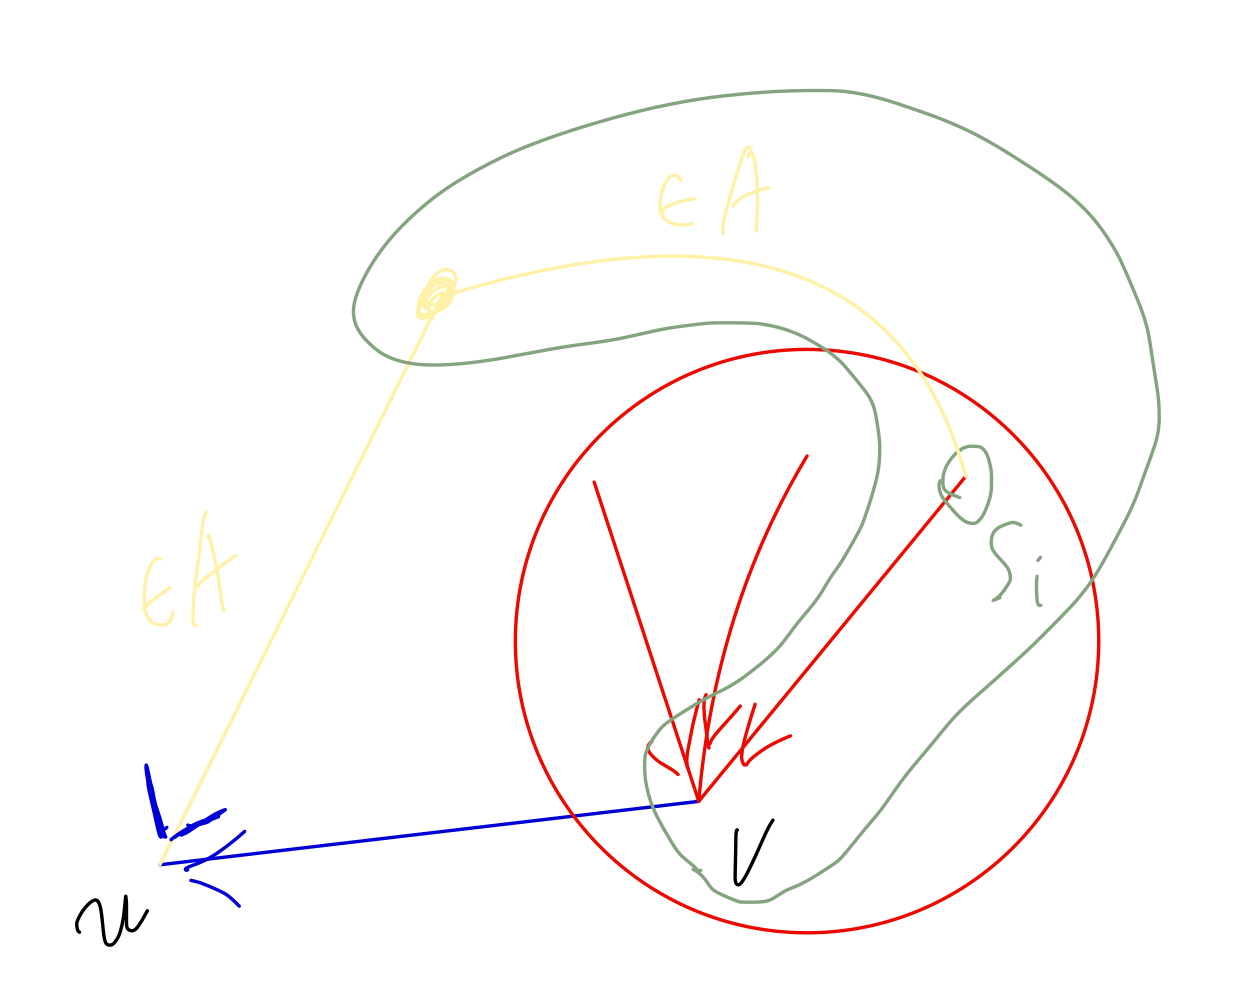
\includegraphics[width=0.5\linewidth]{figures/proof_spanning_oriented_cluster_yellow.jpeg}
  	\caption{Existence of path of length 3 from any $v$ with high degree.}
  	\label{fig:proof_spanning_oriented_cluster_yellow}
  \end{figure}

  So, because there is exists $(v, u) \in E(\vec G \setminus B)$, then there is some vertex from cluster of $v$ such that we added edge from it to $u$.

  We would use \ref{df:hitting_sets} with parameter $k \approx O(\frac{n}{q} \log n)$(here, $t$ is a multiplication of count of vertices and updates in stream, hence polynomial of $n$), where hitting sets in our case is for every $v$ with high degree we took all vertices that has edges to $v$ in $\vec G$.
  Because we have a stream, it would be crucial to suppose that stream is fixed(but we just don't know it) and that our random hitting set would still work for entire stream.

  We construct $B$ as follows, take vertex $u$ and put $q$ \textbf{out} edges from $\vec G$ with minimum lexicographical end to $B$.
  See Fig. \ref{fig:proof_spanning_b_out}.

  \begin{figure}[H]
  	\centering
  	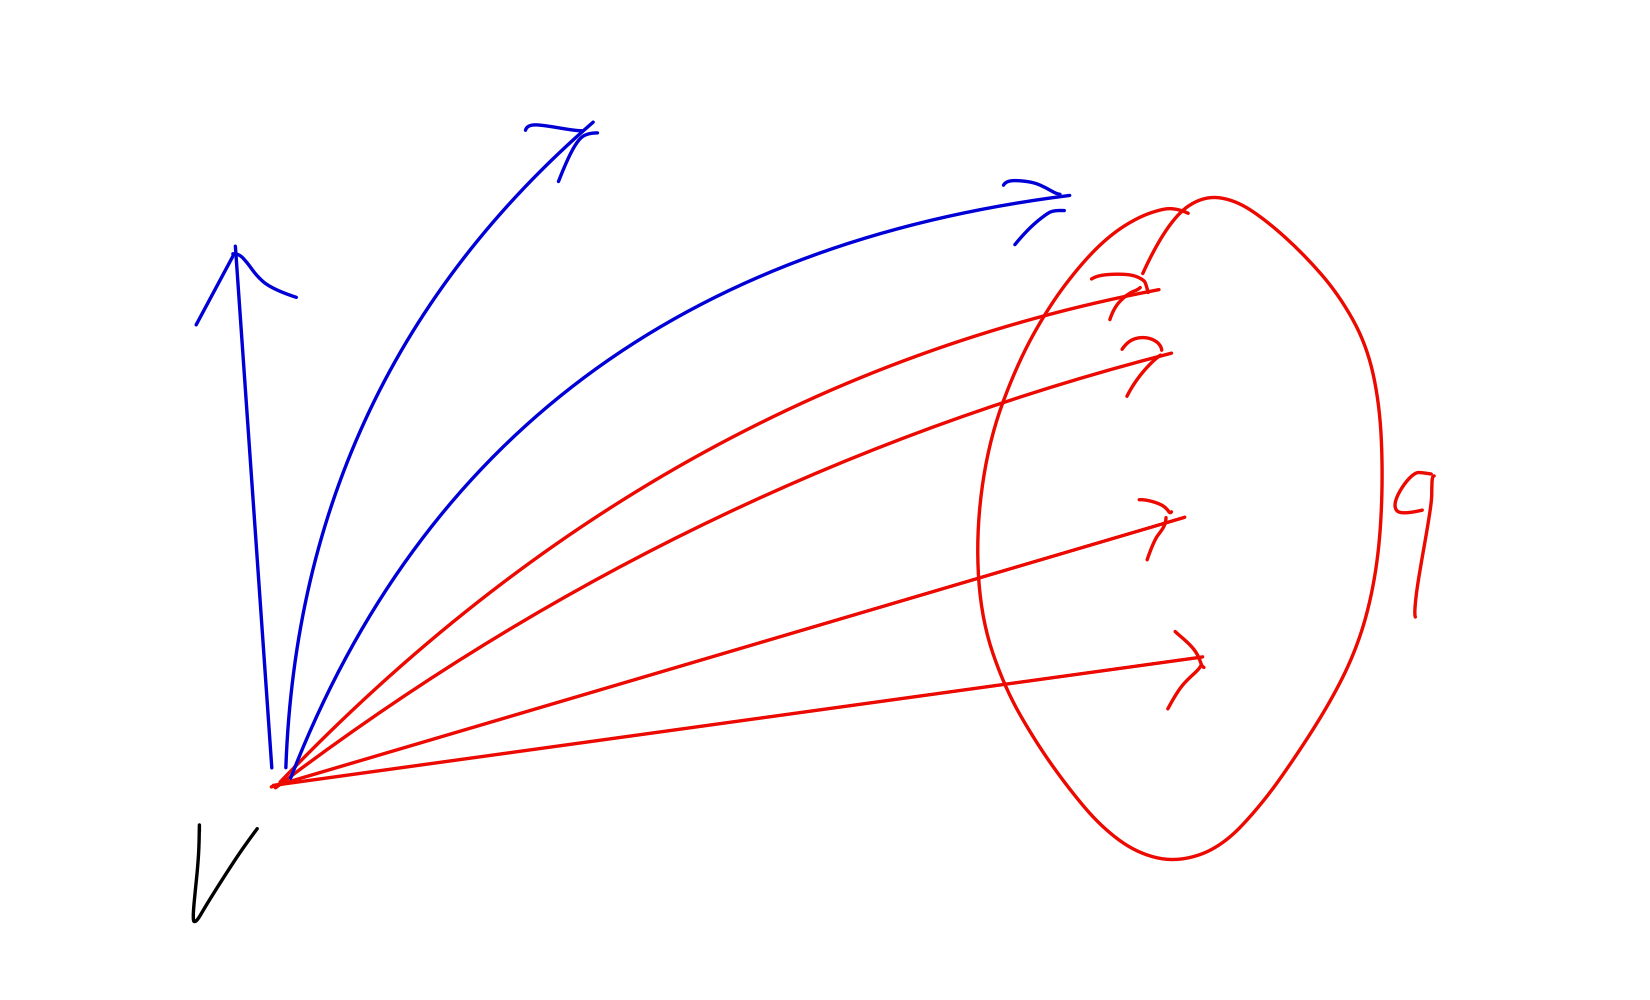
\includegraphics[width=0.4\linewidth]{figures/proof_spanning_b_out.jpeg}
  	\caption{Take first $q$ out edges from $\vec G$ and put them to $B$.}
  	\label{fig:proof_spanning_b_out}
  \end{figure}

  Now take any edge $(v, u) \in \vec G$.
  Implies, that or $(v, u) \in B$, or $\deg^{out}_{\vec G}(v) > q$.
  In second case there is a path of length 3. And hence $A$ is a 3-spanner for $G - \tilde B$.

  Amount of edges in $A$ is no more than $n + n \cdot k$, first is edge to cluster center and second from vertex to any other cluster.
  Edges in $B$ is $n q$, so edges in $H$ is 

  \begin{align*}
	  nk + nq = O\left(\frac{n^2}{q} \log n + n q\right) = [q = \sqrt{n \log n}] = O\left(n^{\frac{3}{2}} \sqrt {\log n}\right)
  \end{align*}

  To make $5$-spanner we would take one minimal edge from one cluster to another in $A$. And in $B$ also put $q$ in edges.
  See Fig. \ref{fig:proof_spanning_5}.

\begin{figure}[H]
	\centering
	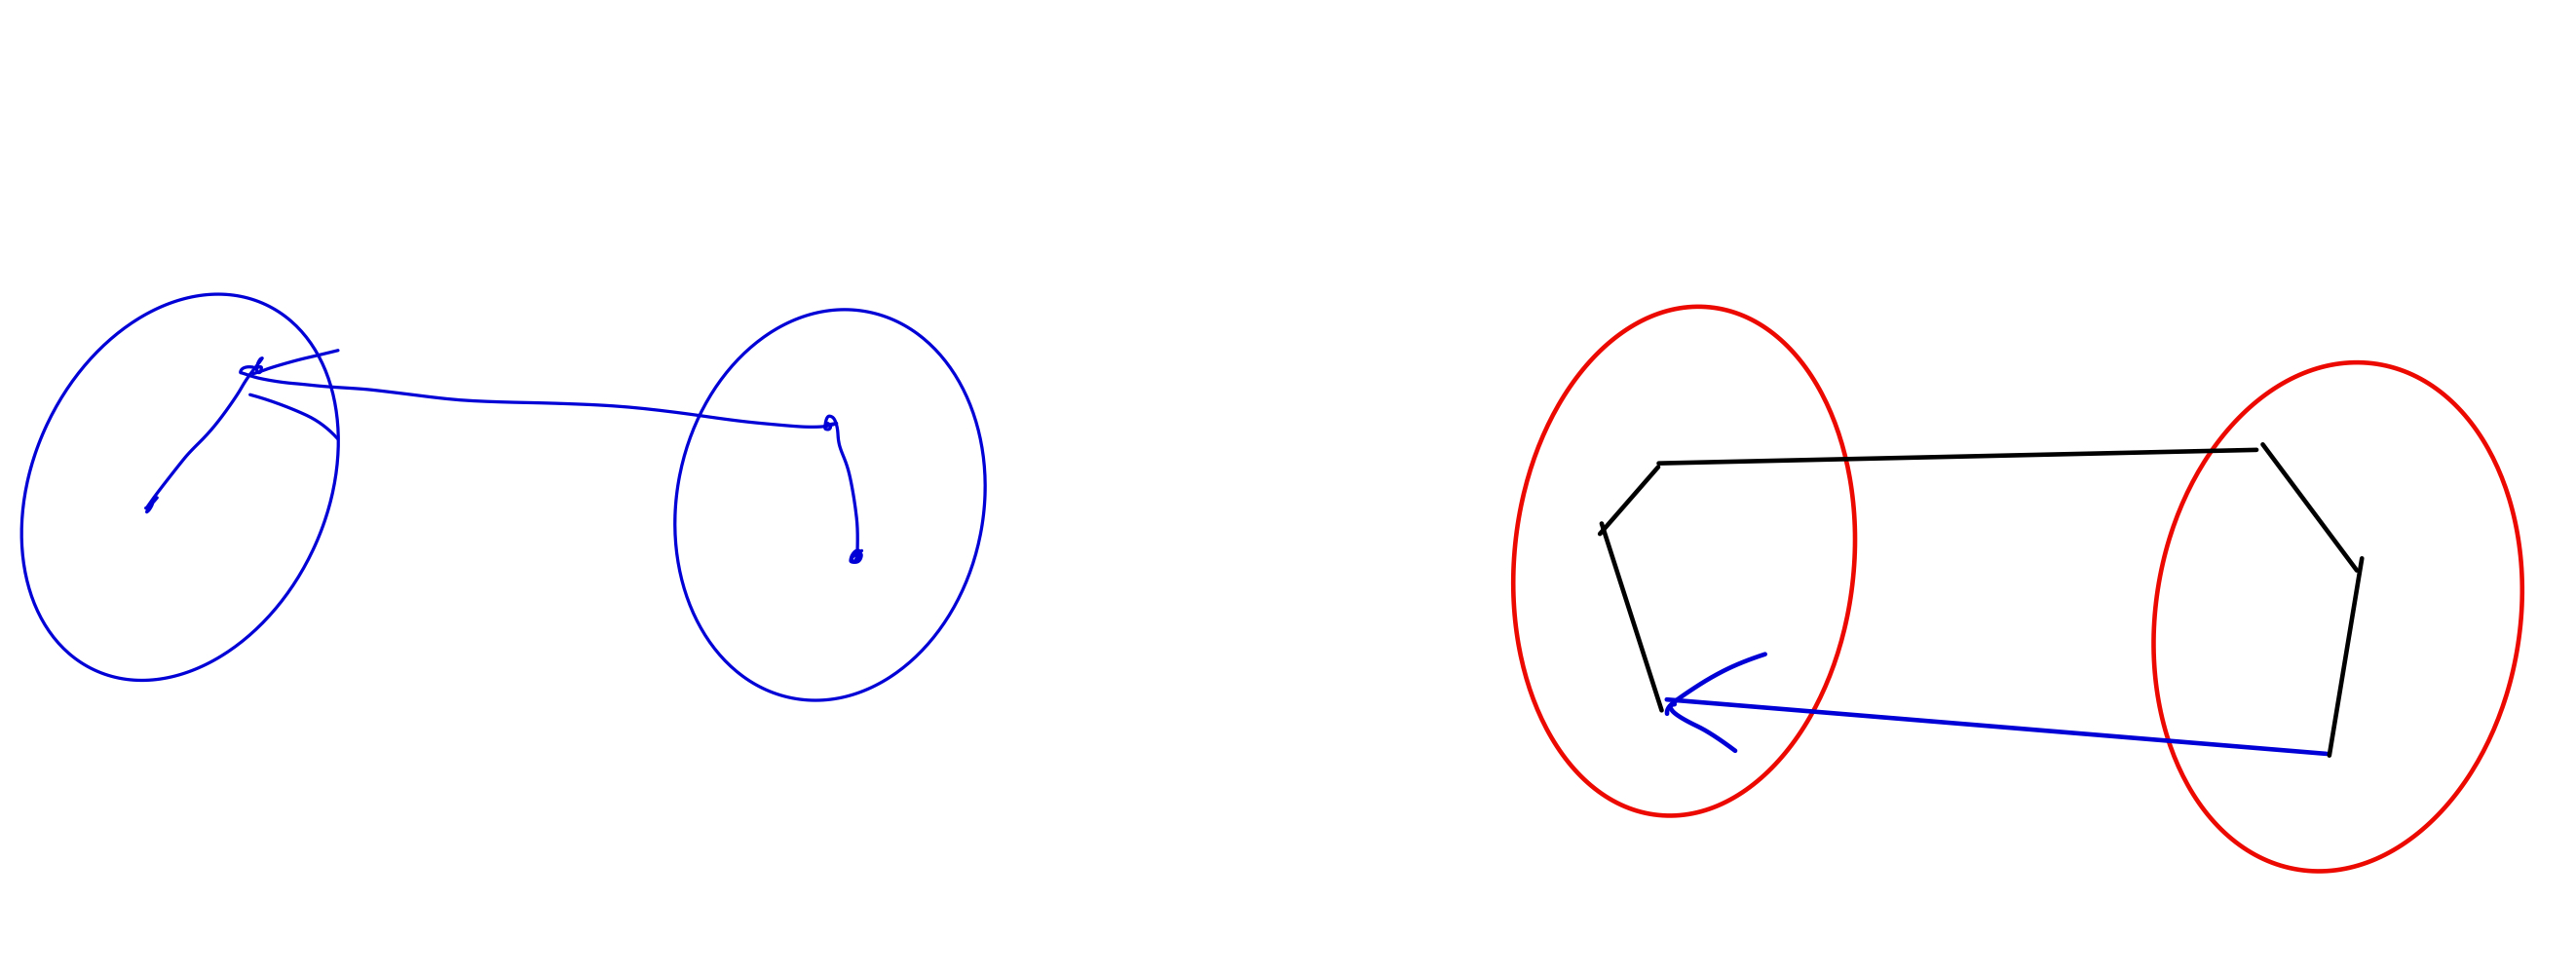
\includegraphics[width=0.7\linewidth]{figures/proof_spanning_5.jpeg}
	\caption{Edges in 5-spanning. On left we put an edge between any two clusters(only one edge). On the right every blue edge from $\vec G$ can be changed to 4 edges inside clusters and one between two clusters.}
	\label{fig:proof_spanning_5}
\end{figure}

  And we would have
  \begin{align*}
    k^2 + nq = \frac{n^2}{q^2} \log n + nq \approx O\left(n^{\frac{4}{3}}\right)
  \end{align*}

  Now we would adapt our $3$-spanning to streaming.

  On edge deletion.
  To keep $B$: when deleting red we put next minimal black. On deleting black we do nothing.
  See Fig. \ref{fig:proof_spanning_delete_b}.

  \begin{figure}[H]
  	\centering
  	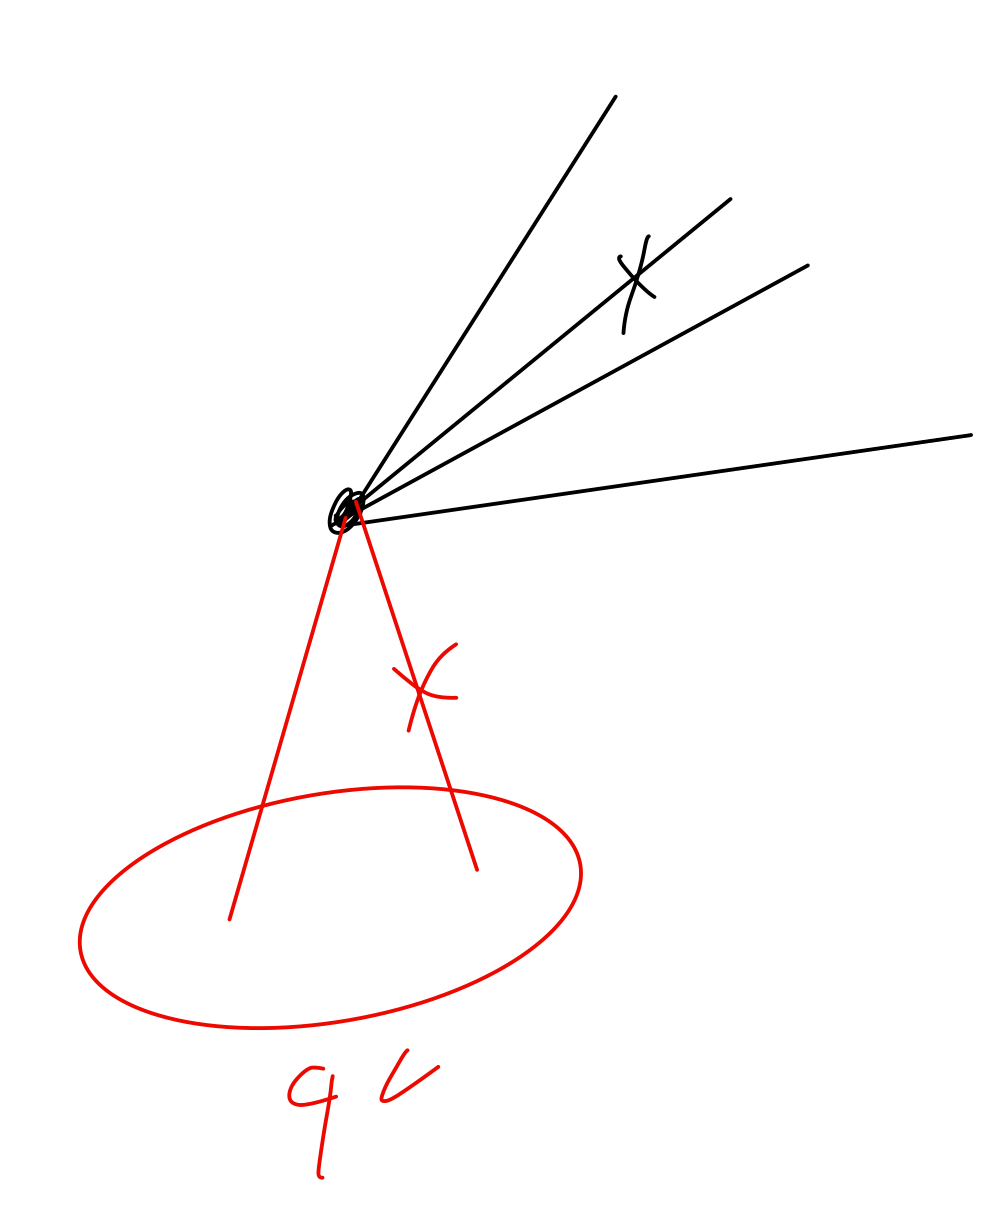
\includegraphics[width=0.3\linewidth]{figures/proof_spanning_delete_b.jpeg}
  	\caption{Deleting edge from $B$.}
  	\label{fig:proof_spanning_delete_b}
  \end{figure}

  To keep A:
  If we delete edge to connecting to center of cluster we can fast find a new cluster center(if it exists).
  See Fig. \ref{fig:proof_spanning_delete_cluster_center}.

	\begin{figure}[H]
		\centering
		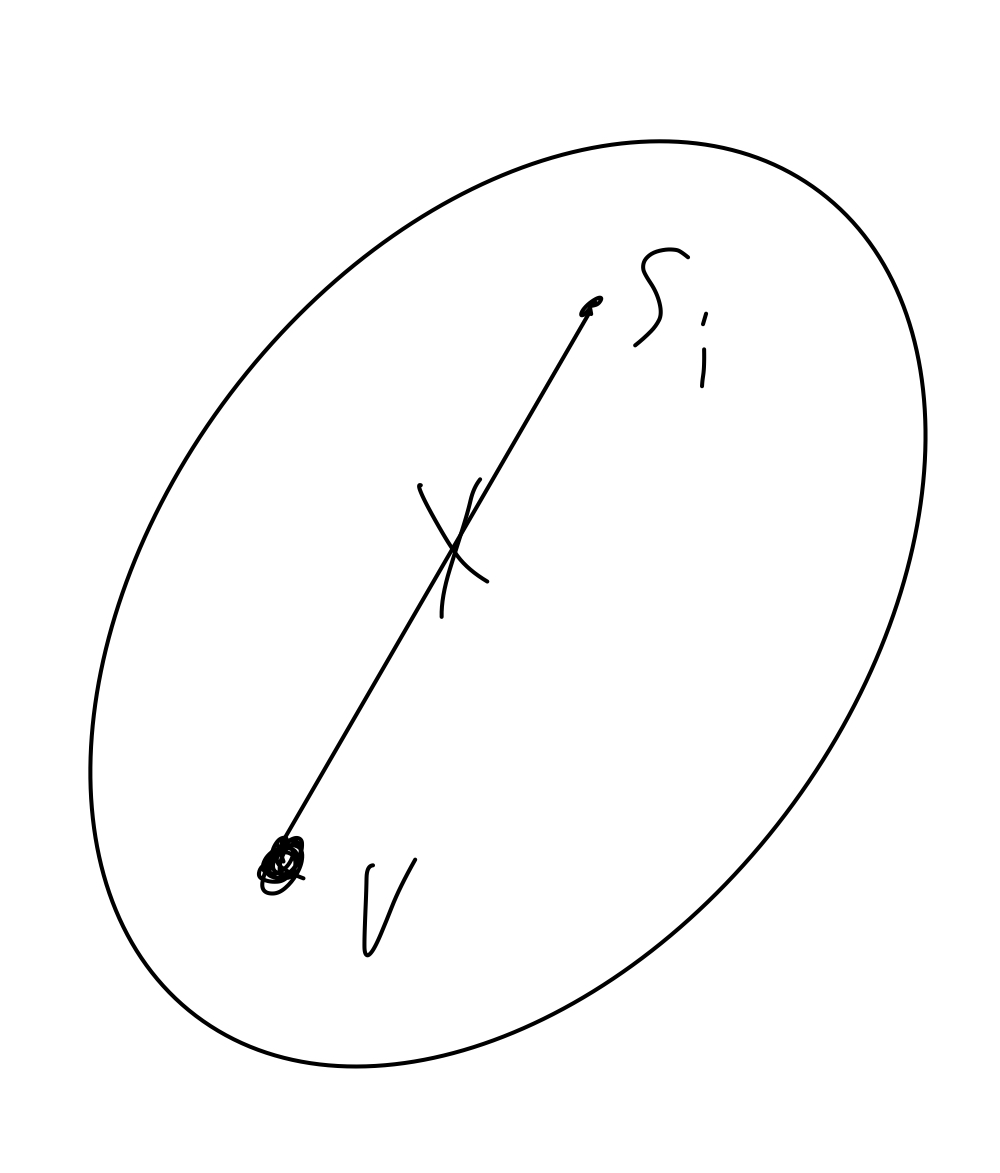
\includegraphics[width=0.3\linewidth]{figures/proof_spanning_delete_cluster_center.jpeg}
		\caption{Delete an edge to cluster center.}
		\label{fig:proof_spanning_delete_cluster_center}
	\end{figure}

	Also vertex can add red edges. We should find for each of those red new vertex from cluster $C_i$.
	And maybe new black edges would be red.
	See Fig. \ref{fig:proof_spanning_add_red_after_delete}.

	\begin{figure}[H]
		\centering
		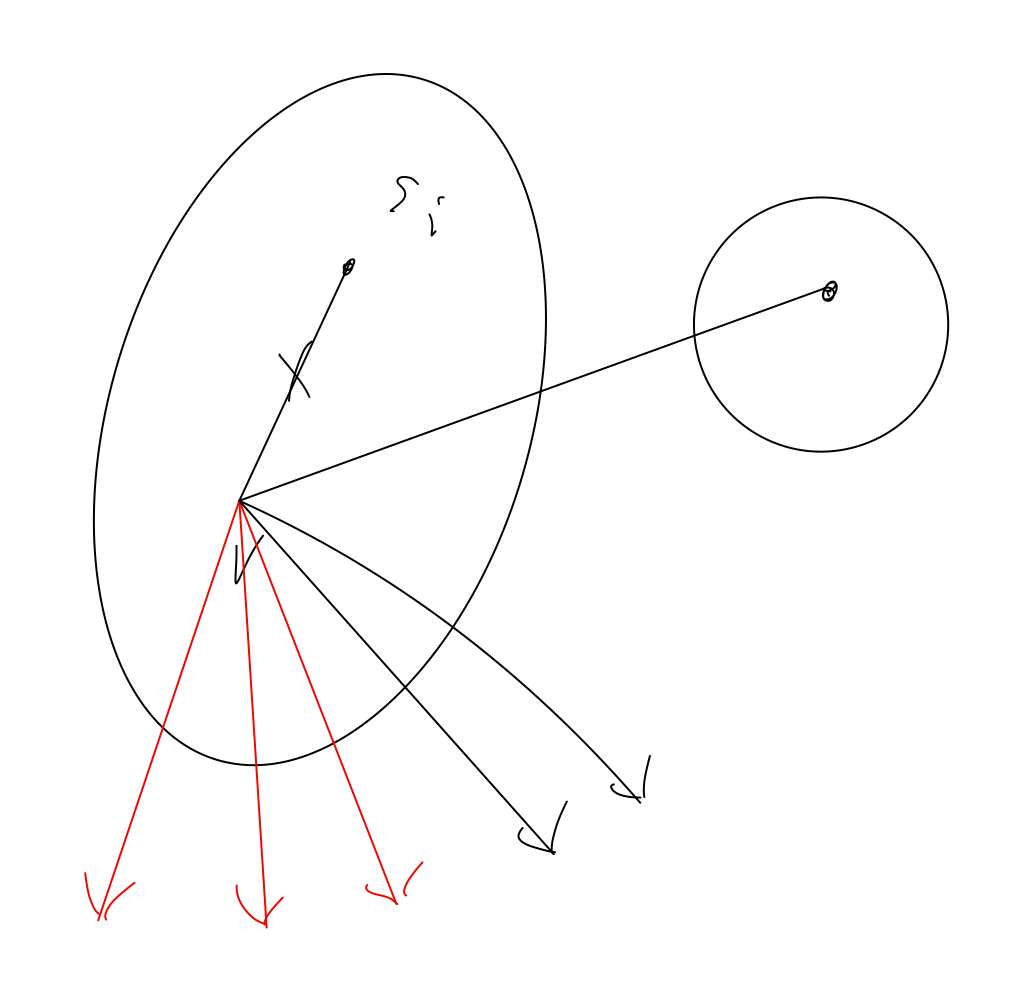
\includegraphics[width=0.5\linewidth]{figures/proof_spanning_add_red_after_delete.jpeg}
		\caption{Deleting red edges and finding new reds.}
		\label{fig:proof_spanning_add_red_after_delete}
	\end{figure}

	Such update we do in time $O\left(\deg_{\vec G}^{out}(v) \log n\right)$. So now, each update can take up to $n \log n$ time.

	\end{proof}

	\begin{lm}[Alg2] \label{lm:spanning_alg_2}
	  There exists an algorithm that returns $A$ and $B$ and process each update in time $O(s \log n)$ and every update change $B$ $O(1)$ times.
	\end{lm}
	\begin{proof}
	  

	Plan: split $G$ into subgraphs of small degree.
	Spanners has property such that if $G = G_1 \cup G_2$ and if we have spanners for $H_1, H_2$ for $G_1, G_2$, respectively. Then $H = H_1 \cup H_2$ is a spanner for $G$.

	Let's take our graph $G$ and split it into substreams. 
	And construct our $A, B$ for each of them.
	And our resulting spanner would be $\bigcup$ of all of them.

	So $|A| = O\left(\frac{\Delta^+(\vec G) n^2 \log n}{s q}\right)$, where $\delta^+$ is a maximal out degree.
	Where $A$ is a 3-spanning for $G \setminus \tilde B$.

	And $\Delta^+(B) \leq \frac{\Delta^+(\vec G)} {s} q$.


	We would have $\frac{\Delta^+(\vec G)}{s} = t$ groups for some parameter $s$(splitting edges into groups and each group gives us a graph).
	They gives us $G_1, \ldots, G_t$.

	And we want have $\Delta^+(\vec G_i)) \leq s$.

	On each new edge we put it into graph to satisfy condition $\Delta^+(\vec G_i) \leq s$.
	We have immediately estimation of size $A$.

	\end{proof}

	Let's move to final phase of our algorithm.

	We would have a sequence of $B$'s and $A$'s.

	\begin{align*}
		B_0 &= \vec G \\
		(B_i, A_i) &\gets \text{Alg2}(\underbrace{B_{i - 1}}_{\text{graph}}, s, \underbrace{q_{i - 1}}_{\text{clusters}}) && i \in 1 \dots l.
	\end{align*}, so $l$ is a amount of steps of our algorithm. And Alg2 defined in Lemma \ref{lm:lm:spanning_alg_2}. And we treat updates in $i$th level of $B_i$ as a new stream to Alg2 for $i + 1$, so size of stream grows exponentially.

	And hence $H = \text{Alg1}(B_l) \cup \bigcup_{i = 1}^{l} A_l$, where Alg1 defined in Lemma \ref{lm:spanning_alg_1}.

	What's going on?

	We had $\vec G$, after that we have $A_1, B_1$ where $A_1$ is a 3-spanner of $G \setminus \tilde B_1$.
	Implies we need a spanner for $B_1$.
	And in asymptotic of Alg2 to make $|A|$ small we should take big $q$. And we would take such $s$ to decrease $\Delta^+(B)$ fast.

	Obviously, 
	\begin{align*}
		\Delta^+(B_j) \leq n \prod_{i = 1}^j \frac{q_j}{s}
	\end{align*}, hence
	\begin{align*}
		|H| = |H'| + \sum_{i = 1}^{l} |A_i| &= O\left(n^{\frac{3}{2}} \sqrt{\log n}\right) + \sum_{i = 1}^{l} \frac{\Delta^+(B_{j - 1}) n^2 \log n}{ s q_j } = \\
											&= [\text{some constants}] = O\left(n^{\frac{3}{2}} \sqrt{\log n} \log \log n\right)
	\end{align*}

	See constants below:

	\begin{figure}[H]
		\centering
		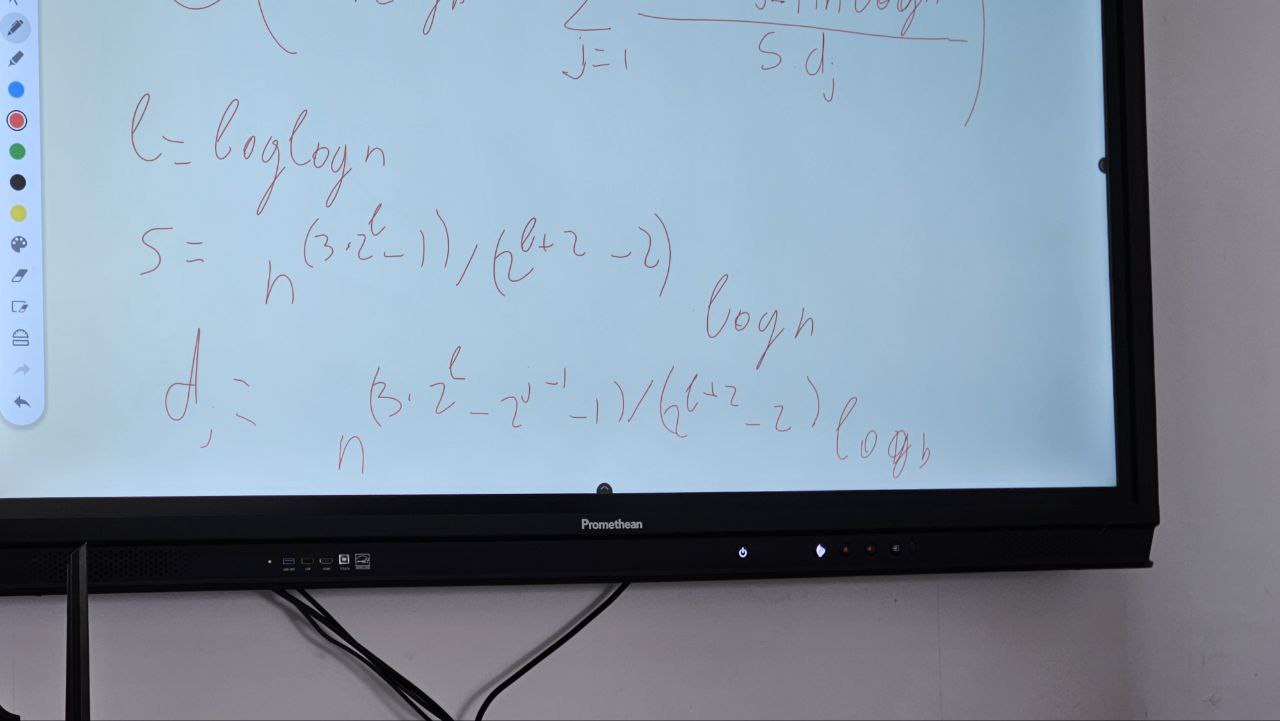
\includegraphics[width=0.5\linewidth]{figures/proof_spanning_contants.jpg}
		\caption{Hah}
		\label{fig:proof_spanning_contants}
	\end{figure}

	Update time:
	\begin{align*}
		O\left(\left(4^{l} \Delta^+(B_l) + \sum_{j = 0}^{l - 1} 4^{j}s\right)\log n\right) = O\left(n^{\frac{3}{4}} (\log n)^{4}\right)
	\end{align*}


\end{proof}

\begin{remrk}
  To remove limitation on polynomial size of a stream($4n^3$) we can hold two graphs $G_1$ and $G_2$, where $G = G_1 \cup G_2$ and we would first half of polynomial steps fit in $G_1$ and after that for half more polynomial steps add new things to $G_2$ and also remove one edge from $G_1$ and add it to $G_2$. After polynomial steps we make it back from $G_2$ to $G_1$.
\end{remrk}

